\documentclass{article}

\usepackage[main=english,vietnamese]{babel}
\usepackage[T1]{fontenc}
\usepackage[utf8]{inputenc}
\usepackage[sexy]{evan}
\usepackage{matchsticks}
\usepackage{wrapfig}
\usepackage{listings}

\newtheorem{hint}{Hint}

\title{Some advanced counting techniques}
\author{Nghia Doan}
\date{\today}

\begin{document}

\maketitle

\begin{definition*}[Set]
    A set is \textit{a collection of objects.}
    
    There might only be a \textit{finite} number of objects in the set, so we could count them if we like,
    in which case the set is called a finite set. Otherwise we call it an \textit{infinite} set.

    The objects in the set are called the \textit{elements or members} of the set.

    The set with no elements at all is called the \textit{empty set,} denoted by $\emptyset$. 
\end{definition*}

\begin{definition*}[Supersets \& Subsets]
    A set $A$ is called a \textit{subset} of a set $B$ if every element of $A$ is also an element of $B,$ denoted by
    \[
        A \subseteq B
    \]
    If $A$ is a subset of $B$, we also say that $B$ is a \textit{superset} of $A$.
\end{definition*}

\begin{definition*}[Intersections \& Unions]
    The \textit{union} $A \cup B$ of two sets $A$ and $B$  is the set of all objects that are elements of $A$ or of $B,$
    \[
        A \cup B = \{x \;|\; x \in A \text{ or } x \in B\}.
    \]
   
    The \textit{intersection} $A \cap B$ of two sets $A$ and $B$ is the set of all objects that are elements of both $A$ and $B,$
    \[
        A \cap B = \{x \;|\; x \in A \text{ or } x \in B\}.
    \]
\end{definition*}

\begin{definition*}[Disjoint]
    If $A \cap B = \emptyset$, then we say that $A$ and $B$ are \textit{disjoint}. 
\end{definition*}

\begin{definition*}[Difference]
    The set difference of two sets $A$ and $B$ is 
    \[
        A \setminus B = \{x \in A \;|\; x \not\in B \}.
    \]
\end{definition*}

\begin{definition*}[Cardinality]
    For a set $S,$ $|S|$ denotes the \textbf{cardinality} of $S,$
    in other words the number of elements in $S,$
    \textit{for example $|\{1, 3, 5, 7\}| = 4.$} The \textbf{empty} set is denoted by $\emptyset.$
\end{definition*}

\begin{theorem*}[The Principle Inclusion-Exclusion for two/three sets]
    \label{theorem:inclusion-exclusion-principle}
    If $A$ and $B$ are two sets, then 
    \[ 
        |A \cup B| = |A| + |B| - |A \cap B|.
    \] 
    If $A$, $B$, and $C$ are three sets, then 
    \[
        |A \cup B \cup C| = |A| + |B| + |C| - |A \cap B| - |A \cap C| - |B \cap C| + |A \cap B \cap C|
    \]
\end{theorem*}

\newpage

\begin{example}[Example One]
    In how many rearrangements of the numbers $1, 2, 3, 4, 5, 6, 7, 8, 9$ do the numbers form a \textit{hill,}
    that is, the numbers form an increasing sequence at the beginning up to a peak,
    and then form a decreasing sequence to the end such as in $129876543$ or $258976431$?
\end{example}

\begin{soln}
    Since in any such arrangement the number 9 must be the number of the peak,
    the numbers in the arrangement must increase to the position of the 9, and then decrease after that position.

    The sequence is then \textit{completely determine by the numbers that come before the 9.}
    There are $2^8$ subsets of $\{1, 2, 3, 4, 5, 6, 7, 8\}$ that could make up the numbers that come before the 9,
    except that neither the empty set or the entire set result in an arrangement that both increase up to 9 and decrease after 9.

    Therefore, there are $2^8 - 2 = \boxed{254}$ possible sequences that form a \textit{hill.}
\end{soln}

\begin{example}[Example Two]
    Find the least six-digit palindrome that is a multiple of 45.
    Note that a palindrome is a number that reads the same forward and backwards such as 1441 or 35253.
\end{example}

\begin{soln}
    A number is a multiple of 45 exactly when it is a multiple of both 5 and 9. 
    
    The decimal representation of a number divisible by 5 must end in the digit 0 or 5.
    A six-digit palindrome cannot end in 0.

    A number is a multiple of 9 if the sum of its digits is a multiple of 9.
    A six-digit palindrome must have the sum of its digits as a multiple of 18 since each of its digits appears twice.
    
    The least such six-digit palindrome must then start with 5, follow by a pair of two digits adding up to 4, then another 5.
    The least such number is $\boxed{504405.}$
\end{soln}

\begin{example}[Example Three]
    How many four-digit positive integers have no adjacent equal even digits? For example, count numbers such as 1164 and 2035 but not 6447 or 5866.
\end{example}

\begin{soln}
    There are $9999 - 999 = 9000$ four-digit positive integers.
    
    Let $A$ be the set of four-digit positive integers where the first two digits are the same even digits,
    $B$ be the set of four-digit positive integers where the second and third digits are the same even digits,
    $C$ be the set of four-digit positive integers where the last two digits are the same even digits.

    Thus we count four-digit positive integers have no adjacent equal even digits, or
    \[
        9000 - |A \cup B \cup C|.
    \]

    By the \nameref{theorem:inclusion-exclusion-principle}, 
    \[
        |A \cup B \cup C| = |A| + |B| + |C| - |A \cap B| - |B \cap C| - |C \cap A|+ |A \cap B \cap C|.
    \]

    Now it is easy to find that for any number in $A,$ there are 4 choices for the first (and second) digits: $2,4,6,8$
    and $10$ choices for the third or the fourth choices, thus $|A| = 4 \cdot 100.$ Similarly,
    \[
        |B| = 5 \cdot 90, |C| = 5 \cdot 90, 
        |A \cap B| = 4 \cdot 10, |B \cap C| = 5 \cdot 9, |A \cap C| = 4\cdot 5, |A \cap B \cap C| = 4.
    \]

    Then $|A \cup B \cup C| = (400+450+450)-(40+45+20)+4 = \boxed{1199.}$
\end{soln}

\begin{example}[Example Four]
    In how many ways can the letters in the word MEMENTO be arranged
    if no two of the same letter may appear consecutively in an arrangement?
\end{example}

\begin{soln}
    Let use the \nameref{theorem:inclusion-exclusion-principle} to solve this problem.

    The total number of arrangement is $A=\frac{7!}{2!}{2!}.$

    The number of ways for the two $M$s to appear consecutively is $B=\frac{6!}{2!}$ because the $MM$ block can be seen as a single letter. 
    Similarly there are $B=\frac{6!}{2!}$ ways for two $E$s to be together. 
    
    Furthermore there are $C=5!$ ways to arrange if both letter $M$s and  both letter $E$s appear together.

    The total number of ways no two $M$s or two $E$s appear together is \textit{the total number of arrangement
    subtracts the number of ways for the two $M$s to appear consecutively, then subtracts the number ways for two $E$s to be together,
    then adds back the number of ways to arrange if both letter $M$s and  both letter $E$s appear together,} or
    \[
        A-2B+C=\frac{7!}{2!}{2!}-2\frac{6!}{2!}+5!=\boxed{660.}
    \]
\end{soln}

\begin{example}[Example Five]
    How many 6-digit numbers, written in decimal notation, have at least one 1, one 2, and one 3 among their digits?
\end{example}

\begin{soln}
    Let $S_1$, $S_2$, and $S_3$ be the sets of 6-digit numbers that do not contain the digits 1, 2, and 3, respectively.
    Then by \nameref{theorem:inclusion-exclusion-principle}, the number of 6-digit numbers that are missing at least one of the digits 1, 2, or 3 is
    \[
        |S_1 \cup S_2 \cup S_3| = |S_1| + |S_2| + |S_3| - |S_1 \cap S_2|- |S_1 \cap S_3| - |S_2 \cap S_3| + |S_1 \cap S_2 \cap S_3|
    \]

    First we count $|S_1|$, the number of 6-digit numbers that do not contain the digit 1.
    The first digit has 8 possible values (2 through 9), and each of the remaining 5 digits has 9 possible values,
    so $|S_1 = 8 \cdot 9^5$. Similarly, $|S_2| = |S_3| = 8 \cdot 9^5$.

    Next we count $|S_1 \cap S_2|$, the number of 6-digit numbers that do not contain the digit 1 or 2.
    The first digit has 7 possible values (3 through 9), and each of the remaining 5 digits has 8 possible values,
    so $|S_1 \cap S_2| = 7 \cdot 8^5$. Similarly, 
    \[ 
        |S_1 \cap S_3| = |S_2 \cap S_3| = 7 \cdot 8^5.
    \]

    Finally, we count $|S_1 \cap S_2 \cap S_3|$, the number of 6-digit numbers that do not contain the digits 1, 2, or 3.
    The first digit has 6 possible values (4 through 9), and each of the remaining 5 digits has 7 possible values,
    so $|S_1 \cap S_2 \cap S_3| = 6 \cdot 7^5$.

    Therefore, $|S_1 \cup S_2 \cup S_3| = 3 \cdot 8 \cdot 9^5 - 3 \cdot 7 \cdot 8^5 + 6 \cdot 7^5 = 829\ 890.$
    
    There are a total of $9 \cdot 10^5 = 900\ 000$ 6-digit numbers,
    so there are $900\ 000 - 829\ 890 = \boxed{70\ 110}$ 6-digit numbers that have at least one 1, one 2, and one 3.
\end{soln}

\begin{example}[Example Six]
    How many subsets of $\{1, 2, 3, 4, 5, 6, 7, 8, 9, 10, 11, 12\}$
    have the property that no two of its elements differ by more than $5$?
    For example, count the subsets $\{3\}$, $\{2, 5, 7\}$, and $\{5, 6, 7, 8, 9\}$
    but not the subset $\{1, 3, 5, 7\}.$
\end{example}

\begin{soln}
    Let $S$ be a subset such that no two of its elements differ by more than $5$.
    Obviously the empty set is such a subset.
    Let consider non-empty subset $S$. Because $S$ has a finite number of element, so there exists 
    the smallest element $e \in S$.

    \textit{Case 1:} $1 \le e \le 7$, any element from $e+1,\ e+2,\ \ldots,\ e+5$ can be element of $S$.
    So there are $7\cdot 2^5=224$ ways to choose from those number to form $S$ (together with $e$).

    \textit{Case 2:} $8\le e \le 12$, for each $e$, there are $12-e$ elements larger than $e$.
    From the previous case, there are $2^{12-e}$ ways to choose from those number to form $S$ (together with $e$).
    It means the number of ways for this case is $2^4+2^3+2^2+2^1+2^0=31.$

    Thus, the number of such subsets is $1+224+31=\boxed{256.}$
\end{soln}

\begin{example}[Example Seven]
    Residents were surveyed in order to determine which flowers to plant in the new Public Garden.
    A total of $N$ people participated in the survey.
    Exactly $\frac{9}{14}$ of those surveyed said that the colour of the flower was important.
    Exactly $\frac{7}{12}$ of those surveyed said that the smell of the flower was important.
    In total, $753$ people said that both the colour and smell were important.
    How many possible values are there for $N$?
\end{example}

\begin{soln}
    The difficulty of the problem is that the quantities are given as fractions of unknown value $N.$
    Our approach is to \textit{turn $N$ into a multiple of the least common multiple of the denominators} of the fractions.
    This ways the fractions can be transformed into integer variables.
    The rest is based \textit{using a Venn-diagram to estimate},
    \begin{enumerate}[topsep=0pt, partopsep=0pt, itemsep=0pt]
        \ii the lowest value of $k$ based on the number of common people in both sets, and
        \ii the highest value of $k$ based on the number of people not in any of the sets.
    \end{enumerate}

    \begin{center}
        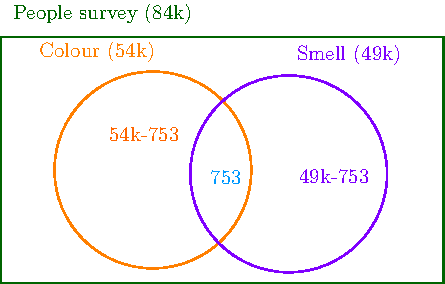
\includegraphics[width=7.5cm]{./asy/pdf/gauss-g8-2014-25.pdf}
    \end{center}

    Since the least common multiple of the denominator $\text{lcm}(12,14)=84,$ thus $84 \mid N.$
    Let $N=84k,$ where $k$ is a positive integer.

    \textit{The minimum value of $k$}, since $753$ is the number of people in both sets, so
    \[
        \begin{cases}
            54k - 753 \ge 0\\
            49k - 753 \ge 0
        \end{cases}
        \Rightarrow 49k - 753 \ge 0 \Rightarrow k \ge 16
    \]

    \textit{The maximum value of $k$}, the number of people outside of both sets is
    \[
        84k - (54k - 753) - (49k - 753) - 753 = 753 - 19k \ge 0 \Rightarrow k \le 39
    \]

    It is easy to see that all values of $k$ between $16$ and $39,$ including both $16$ and $39,$ satisfy the given conditions.
    Thus there are \framebox{$39-16+1=24$} such values.
\end{soln}

\end{document}